\documentclass[1p]{elsarticle_modified}
%\bibliographystyle{elsarticle-num}

%\usepackage[colorlinks]{hyperref}
%\usepackage{abbrmath_seonhwa} %\Abb, \Ascr, \Acal ,\Abf, \Afrak
\usepackage{amsfonts}
\usepackage{amssymb}
\usepackage{amsmath}
\usepackage{amsthm}
\usepackage{scalefnt}
\usepackage{amsbsy}
\usepackage{kotex}
\usepackage{caption}
\usepackage{subfig}
\usepackage{color}
\usepackage{graphicx}
\usepackage{xcolor} %% white, black, red, green, blue, cyan, magenta, yellow
\usepackage{float}
\usepackage{setspace}
\usepackage{hyperref}

\usepackage{tikz}
\usetikzlibrary{arrows}

\usepackage{multirow}
\usepackage{array} % fixed length table
\usepackage{hhline}

%%%%%%%%%%%%%%%%%%%%%
\makeatletter
\renewcommand*\env@matrix[1][\arraystretch]{%
	\edef\arraystretch{#1}%
	\hskip -\arraycolsep
	\let\@ifnextchar\new@ifnextchar
	\array{*\c@MaxMatrixCols c}}
\makeatother %https://tex.stackexchange.com/questions/14071/how-can-i-increase-the-line-spacing-in-a-matrix
%%%%%%%%%%%%%%%

\usepackage[normalem]{ulem}

\newcommand{\msout}[1]{\ifmmode\text{\sout{\ensuremath{#1}}}\else\sout{#1}\fi}
%SOURCE: \msout is \stkout macro in https://tex.stackexchange.com/questions/20609/strikeout-in-math-mode

\newcommand{\cancel}[1]{
	\ifmmode
	{\color{red}\msout{#1}}
	\else
	{\color{red}\sout{#1}}
	\fi
}

\newcommand{\add}[1]{
	{\color{blue}\uwave{#1}}
}

\newcommand{\replace}[2]{
	\ifmmode
	{\color{red}\msout{#1}}{\color{blue}\uwave{#2}}
	\else
	{\color{red}\sout{#1}}{\color{blue}\uwave{#2}}
	\fi
}

\newcommand{\Sol}{\mathcal{S}} %segment
\newcommand{\D}{D} %diagram
\newcommand{\A}{\mathcal{A}} %arc


%%%%%%%%%%%%%%%%%%%%%%%%%%%%%5 test

\def\sl{\operatorname{\textup{SL}}(2,\Cbb)}
\def\psl{\operatorname{\textup{PSL}}(2,\Cbb)}
\def\quan{\mkern 1mu \triangleright \mkern 1mu}

\theoremstyle{definition}
\newtheorem{thm}{Theorem}[section]
\newtheorem{prop}[thm]{Proposition}
\newtheorem{lem}[thm]{Lemma}
\newtheorem{ques}[thm]{Question}
\newtheorem{cor}[thm]{Corollary}
\newtheorem{defn}[thm]{Definition}
\newtheorem{exam}[thm]{Example}
\newtheorem{rmk}[thm]{Remark}
\newtheorem{alg}[thm]{Algorithm}

\newcommand{\I}{\sqrt{-1}}
\begin{document}

%\begin{frontmatter}
%
%\title{Boundary parabolic representations of knots up to 8 crossings}
%
%%% Group authors per affiliation:
%\author{Yunhi Cho} 
%\address{Department of Mathematics, University of Seoul, Seoul, Korea}
%\ead{yhcho@uos.ac.kr}
%
%
%\author{Seonhwa Kim} %\fnref{s_kim}}
%\address{Center for Geometry and Physics, Institute for Basic Science, Pohang, 37673, Korea}
%\ead{ryeona17@ibs.re.kr}
%
%\author{Hyuk Kim}
%\address{Department of Mathematical Sciences, Seoul National University, Seoul 08826, Korea}
%\ead{hyukkim@snu.ac.kr}
%
%\author{Seokbeom Yoon}
%\address{Department of Mathematical Sciences, Seoul National University, Seoul, 08826,  Korea}
%\ead{sbyoon15@snu.ac.kr}
%
%\begin{abstract}
%We find all boundary parabolic representation of knots up to 8 crossings.
%
%\end{abstract}
%\begin{keyword}
%    \MSC[2010] 57M25 
%\end{keyword}
%
%\end{frontmatter}

%\linenumbers
%\tableofcontents
%
\newcommand\colored[1]{\textcolor{white}{\rule[-0.35ex]{0.8em}{1.4ex}}\kern-0.8em\color{red} #1}%
%\newcommand\colored[1]{\textcolor{white}{ #1}\kern-2.17ex	\textcolor{white}{ #1}\kern-1.81ex	\textcolor{white}{ #1}\kern-2.15ex\color{red}#1	}

{\Large $\underline{12n_{0130}~(K12n_{0130})}$}

\setlength{\tabcolsep}{10pt}
\renewcommand{\arraystretch}{1.6}
\vspace{1cm}\begin{tabular}{m{100pt}>{\centering\arraybackslash}m{274pt}}
\multirow{5}{120pt}{
	\centering
	\includegraphics[width=112pt]{../../../GIT/diagram.site/Diagrams/png/2219_12n_0130.png}\\
\ \ \ A knot diagram\footnotemark}&
\allowdisplaybreaks
\textbf{Linearized knot diagam} \\
\cline{2-2}
 &
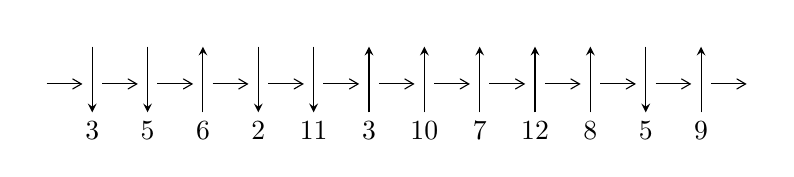
\begin{tikzpicture}[x=20pt, y=17pt]
	% nodes
	\node (C0) at (0, 0) {};
	\node (C1) at (1, 0) {};
	\node (C1U) at (1, +1) {};
	\node (C1D) at (1, -1) {3};

	\node (C2) at (2, 0) {};
	\node (C2U) at (2, +1) {};
	\node (C2D) at (2, -1) {5};

	\node (C3) at (3, 0) {};
	\node (C3U) at (3, +1) {};
	\node (C3D) at (3, -1) {6};

	\node (C4) at (4, 0) {};
	\node (C4U) at (4, +1) {};
	\node (C4D) at (4, -1) {2};

	\node (C5) at (5, 0) {};
	\node (C5U) at (5, +1) {};
	\node (C5D) at (5, -1) {11};

	\node (C6) at (6, 0) {};
	\node (C6U) at (6, +1) {};
	\node (C6D) at (6, -1) {3};

	\node (C7) at (7, 0) {};
	\node (C7U) at (7, +1) {};
	\node (C7D) at (7, -1) {10};

	\node (C8) at (8, 0) {};
	\node (C8U) at (8, +1) {};
	\node (C8D) at (8, -1) {7};

	\node (C9) at (9, 0) {};
	\node (C9U) at (9, +1) {};
	\node (C9D) at (9, -1) {12};

	\node (C10) at (10, 0) {};
	\node (C10U) at (10, +1) {};
	\node (C10D) at (10, -1) {8};

	\node (C11) at (11, 0) {};
	\node (C11U) at (11, +1) {};
	\node (C11D) at (11, -1) {5};

	\node (C12) at (12, 0) {};
	\node (C12U) at (12, +1) {};
	\node (C12D) at (12, -1) {9};
	\node (C13) at (13, 0) {};

	% arrows
	\draw[->,>={angle 60}]
	(C0) edge (C1) (C1) edge (C2) (C2) edge (C3) (C3) edge (C4) (C4) edge (C5) (C5) edge (C6) (C6) edge (C7) (C7) edge (C8) (C8) edge (C9) (C9) edge (C10) (C10) edge (C11) (C11) edge (C12) (C12) edge (C13) ;	\draw[->,>=stealth]
	(C1U) edge (C1D) (C2U) edge (C2D) (C3D) edge (C3U) (C4U) edge (C4D) (C5U) edge (C5D) (C6D) edge (C6U) (C7D) edge (C7U) (C8D) edge (C8U) (C9D) edge (C9U) (C10D) edge (C10U) (C11U) edge (C11D) (C12D) edge (C12U) ;
	\end{tikzpicture} \\
\hhline{~~} \\& 
\textbf{Solving Sequence} \\ \cline{2-2} 
 &
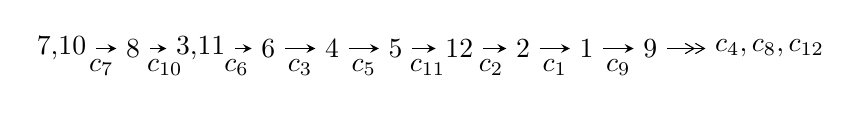
\begin{tikzpicture}[x=23pt, y=7pt]
	% node
	\node (A0) at (-1/8, 0) {7,10};
	\node (A1) at (1, 0) {8};
	\node (A2) at (33/16, 0) {3,11};
	\node (A3) at (25/8, 0) {6};
	\node (A4) at (33/8, 0) {4};
	\node (A5) at (41/8, 0) {5};
	\node (A6) at (49/8, 0) {12};
	\node (A7) at (57/8, 0) {2};
	\node (A8) at (65/8, 0) {1};
	\node (A9) at (73/8, 0) {9};
	\node (C1) at (1/2, -1) {$c_{7}$};
	\node (C2) at (3/2, -1) {$c_{10}$};
	\node (C3) at (21/8, -1) {$c_{6}$};
	\node (C4) at (29/8, -1) {$c_{3}$};
	\node (C5) at (37/8, -1) {$c_{5}$};
	\node (C6) at (45/8, -1) {$c_{11}$};
	\node (C7) at (53/8, -1) {$c_{2}$};
	\node (C8) at (61/8, -1) {$c_{1}$};
	\node (C9) at (69/8, -1) {$c_{9}$};
	\node (A10) at (11, 0) {$c_{4},c_{8},c_{12}$};

	% edge
	\draw[->,>=stealth]	
	(A0) edge (A1) (A1) edge (A2) (A2) edge (A3) (A3) edge (A4) (A4) edge (A5) (A5) edge (A6) (A6) edge (A7) (A7) edge (A8) (A8) edge (A9) ;
	\draw[->>,>={angle 60}]	
	(A9) edge (A10);
\end{tikzpicture} \\ 

\end{tabular} \\

\footnotetext{
The image of knot diagram is generated by the software ``\textbf{Draw programme}" developed by Andrew Bartholomew(\url{http://www.layer8.co.uk/maths/draw/index.htm\#Running-draw}), where we modified some parts for our purpose(\url{https://github.com/CATsTAILs/LinksPainter}).
}\phantom \\ \newline 
\centering \textbf{Ideals for irreducible components\footnotemark of $X_{\text{par}}$} 
 
\begin{align*}
I^u_{1}&=\langle 
3.76813\times10^{29} u^{45}-2.42336\times10^{30} u^{44}+\cdots+4.57009\times10^{29} b-9.07426\times10^{29},\\
\phantom{I^u_{1}}&\phantom{= \langle  }-3.88039\times10^{29} u^{45}+2.51360\times10^{30} u^{44}+\cdots+4.57009\times10^{29} a+2.62337\times10^{30},\;u^{46}-7 u^{45}+\cdots-4 u+1\rangle \\
I^u_{2}&=\langle 
b,\;3 u^8-5 u^7- u^6+9 u^5-6 u^4-3 u^3+10 u^2+a-8 u+4,\;u^9- u^8-2 u^7+3 u^6+u^5-3 u^4+2 u^3- u+1\rangle \\
I^u_{3}&=\langle 
- a^4+6 a^3-9 a^2+b+8 a-3,\;a^5-6 a^4+9 a^3-8 a^2+4 a-1,\;u+1\rangle \\
\\
\end{align*}
\raggedright * 3 irreducible components of $\dim_{\mathbb{C}}=0$, with total 60 representations.\\
\footnotetext{All coefficients of polynomials are rational numbers. But the coefficients are sometimes approximated in decimal forms when there is not enough margin.}
\newpage
\renewcommand{\arraystretch}{1}
\centering \section*{I. $I^u_{1}= \langle 3.77\times10^{29} u^{45}-2.42\times10^{30} u^{44}+\cdots+4.57\times10^{29} b-9.07\times10^{29},\;-3.88\times10^{29} u^{45}+2.51\times10^{30} u^{44}+\cdots+4.57\times10^{29} a+2.62\times10^{30},\;u^{46}-7 u^{45}+\cdots-4 u+1 \rangle$}
\flushleft \textbf{(i) Arc colorings}\\
\begin{tabular}{m{7pt} m{180pt} m{7pt} m{180pt} }
\flushright $a_{7}=$&$\begin{pmatrix}1\\0\end{pmatrix}$ \\
\flushright $a_{10}=$&$\begin{pmatrix}0\\u\end{pmatrix}$ \\
\flushright $a_{8}=$&$\begin{pmatrix}1\\- u^2\end{pmatrix}$ \\
\flushright $a_{3}=$&$\begin{pmatrix}0.849084 u^{45}-5.50010 u^{44}+\cdots+6.33741 u-5.74030\\-0.824518 u^{45}+5.30264 u^{44}+\cdots+0.443856 u+1.98557\end{pmatrix}$ \\
\flushright $a_{11}=$&$\begin{pmatrix}u\\- u^3+u\end{pmatrix}$ \\
\flushright $a_{6}=$&$\begin{pmatrix}0.894837 u^{45}-6.29021 u^{44}+\cdots+2.76162 u-0.388790\\-0.321679 u^{45}+2.27756 u^{44}+\cdots-3.54255 u+1.78782\end{pmatrix}$ \\
\flushright $a_{4}=$&$\begin{pmatrix}-0.151962 u^{45}+1.36037 u^{44}+\cdots+11.0404 u-2.84289\\-1.07500 u^{45}+6.98658 u^{44}+\cdots+0.922265 u+2.06759\end{pmatrix}$ \\
\flushright $a_{5}=$&$\begin{pmatrix}1.14526 u^{45}-7.71445 u^{44}+\cdots+3.87163 u-0.363285\\-0.210798 u^{45}+1.90057 u^{44}+\cdots-3.49688 u+2.14201\end{pmatrix}$ \\
\flushright $a_{12}=$&$\begin{pmatrix}-1.24464 u^{45}+8.36097 u^{44}+\cdots-6.15963 u+4.76903\\-0.0970325 u^{45}+0.230705 u^{44}+\cdots-1.32622 u-1.14760\end{pmatrix}$ \\
\flushright $a_{2}=$&$\begin{pmatrix}-0.625495 u^{45}+4.50917 u^{44}+\cdots+6.85570 u-3.05357\\-0.280998 u^{45}+1.72030 u^{44}+\cdots+4.29468 u+0.101646\end{pmatrix}$ \\
\flushright $a_{1}=$&$\begin{pmatrix}0.760978 u^{45}-5.14121 u^{44}+\cdots+5.63281 u-3.53294\\-0.0351355 u^{45}+0.537169 u^{44}+\cdots+1.00892 u+1.13906\end{pmatrix}$ \\
\flushright $a_{9}=$&$\begin{pmatrix}- u^2+1\\- u^2\end{pmatrix}$\\&\end{tabular}
\flushleft \textbf{(ii) Obstruction class $= -1$}\\~\\
\flushleft \textbf{(iii) Cusp Shapes $= 0.804859 u^{45}-1.44838 u^{44}+\cdots+36.2667 u-15.6976$}\\~\\
\newpage\renewcommand{\arraystretch}{1}
\flushleft \textbf{(iv) u-Polynomials at the component}\newline \\
\begin{tabular}{m{50pt}|m{274pt}}
Crossings & \hspace{64pt}u-Polynomials at each crossing \\
\hline $$\begin{aligned}c_{1}\end{aligned}$$&$\begin{aligned}
&u^{46}+61 u^{45}+\cdots+62504 u+1
\end{aligned}$\\
\hline $$\begin{aligned}c_{2},c_{4}\end{aligned}$$&$\begin{aligned}
&u^{46}-11 u^{45}+\cdots+260 u-1
\end{aligned}$\\
\hline $$\begin{aligned}c_{3},c_{6}\end{aligned}$$&$\begin{aligned}
&u^{46}+8 u^{45}+\cdots+9216 u+512
\end{aligned}$\\
\hline $$\begin{aligned}c_{5},c_{11}\end{aligned}$$&$\begin{aligned}
&u^{46}-3 u^{45}+\cdots+2 u-1
\end{aligned}$\\
\hline $$\begin{aligned}c_{7},c_{10}\end{aligned}$$&$\begin{aligned}
&u^{46}+7 u^{45}+\cdots+4 u+1
\end{aligned}$\\
\hline $$\begin{aligned}c_{8}\end{aligned}$$&$\begin{aligned}
&u^{46}-17 u^{45}+\cdots-22 u+1
\end{aligned}$\\
\hline $$\begin{aligned}c_{9},c_{12}\end{aligned}$$&$\begin{aligned}
&u^{46}+2 u^{45}+\cdots-32 u+32
\end{aligned}$\\
\hline
\end{tabular}\\~\\
\newpage\renewcommand{\arraystretch}{1}
\flushleft \textbf{(v) Riley Polynomials at the component}\newline \\
\begin{tabular}{m{50pt}|m{274pt}}
Crossings & \hspace{64pt}Riley Polynomials at each crossing \\
\hline $$\begin{aligned}c_{1}\end{aligned}$$&$\begin{aligned}
&y^{46}-141 y^{45}+\cdots-3903085204 y+1
\end{aligned}$\\
\hline $$\begin{aligned}c_{2},c_{4}\end{aligned}$$&$\begin{aligned}
&y^{46}-61 y^{45}+\cdots-62504 y+1
\end{aligned}$\\
\hline $$\begin{aligned}c_{3},c_{6}\end{aligned}$$&$\begin{aligned}
&y^{46}+60 y^{45}+\cdots-71827456 y+262144
\end{aligned}$\\
\hline $$\begin{aligned}c_{5},c_{11}\end{aligned}$$&$\begin{aligned}
&y^{46}- y^{45}+\cdots-32 y+1
\end{aligned}$\\
\hline $$\begin{aligned}c_{7},c_{10}\end{aligned}$$&$\begin{aligned}
&y^{46}-17 y^{45}+\cdots-22 y+1
\end{aligned}$\\
\hline $$\begin{aligned}c_{8}\end{aligned}$$&$\begin{aligned}
&y^{46}+31 y^{45}+\cdots+246 y+1
\end{aligned}$\\
\hline $$\begin{aligned}c_{9},c_{12}\end{aligned}$$&$\begin{aligned}
&y^{46}+36 y^{45}+\cdots+8704 y+1024
\end{aligned}$\\
\hline
\end{tabular}\\~\\
\newpage\flushleft \textbf{(vi) Complex Volumes and Cusp Shapes}
$$\begin{array}{c|c|c}  
\text{Solutions to }I^u_{1}& \I (\text{vol} + \sqrt{-1}CS) & \text{Cusp shape}\\
 \hline 
\begin{aligned}
u &= \phantom{-}0.814878 + 0.606452 I \\
a &= \phantom{-}0.433990 - 0.140786 I \\
b &= -0.472583 + 0.137648 I\end{aligned}
 & -2.08149 + 2.37209 I & \phantom{-}0.76660 - 4.29323 I \\ \hline\begin{aligned}
u &= \phantom{-}0.814878 - 0.606452 I \\
a &= \phantom{-}0.433990 + 0.140786 I \\
b &= -0.472583 - 0.137648 I\end{aligned}
 & -2.08149 - 2.37209 I & \phantom{-}0.76660 + 4.29323 I \\ \hline\begin{aligned}
u &= -0.874046\phantom{ +0.000000I} \\
a &= \phantom{-}11.2435\phantom{ +0.000000I} \\
b &= -0.211525\phantom{ +0.000000I}\end{aligned}
 & -0.417366\phantom{ +0.000000I} & \phantom{-}104.440\phantom{ +0.000000I} \\ \hline\begin{aligned}
u &= -1.144360 + 0.047071 I \\
a &= \phantom{-}1.135140 + 0.536251 I \\
b &= -0.050832 - 0.907635 I\end{aligned}
 & \phantom{-}0.67146 - 1.37994 I & -4.76488 + 1.12257 I \\ \hline\begin{aligned}
u &= -1.144360 - 0.047071 I \\
a &= \phantom{-}1.135140 - 0.536251 I \\
b &= -0.050832 + 0.907635 I\end{aligned}
 & \phantom{-}0.67146 + 1.37994 I & -4.76488 - 1.12257 I \\ \hline\begin{aligned}
u &= \phantom{-}0.843227 + 0.031667 I \\
a &= \phantom{-}0.420881 + 0.781766 I \\
b &= -0.461740 - 1.101880 I\end{aligned}
 & -4.57386 + 4.46577 I & -14.2933 - 6.3376 I \\ \hline\begin{aligned}
u &= \phantom{-}0.843227 - 0.031667 I \\
a &= \phantom{-}0.420881 - 0.781766 I \\
b &= -0.461740 + 1.101880 I\end{aligned}
 & -4.57386 - 4.46577 I & -14.2933 + 6.3376 I \\ \hline\begin{aligned}
u &= \phantom{-}0.826663 + 0.817264 I \\
a &= -0.67352 + 1.82579 I \\
b &= \phantom{-}0.460674 + 0.701336 I\end{aligned}
 & -5.00017 + 2.00257 I & \phantom{-}2.00000 - 8.95543 I \\ \hline\begin{aligned}
u &= \phantom{-}0.826663 - 0.817264 I \\
a &= -0.67352 - 1.82579 I \\
b &= \phantom{-}0.460674 - 0.701336 I\end{aligned}
 & -5.00017 - 2.00257 I & \phantom{-}2.00000 + 8.95543 I \\ \hline\begin{aligned}
u &= -1.113100 + 0.352595 I \\
a &= \phantom{-}0.007224 - 0.637262 I \\
b &= \phantom{-}0.601579 - 0.034830 I\end{aligned}
 & \phantom{-}3.69426 - 1.19679 I & \phantom{-}10.96091 + 0. I\phantom{ +0.000000I}\\
 \hline 
 \end{array}$$\newpage$$\begin{array}{c|c|c}  
\text{Solutions to }I^u_{1}& \I (\text{vol} + \sqrt{-1}CS) & \text{Cusp shape}\\
 \hline 
\begin{aligned}
u &= -1.113100 - 0.352595 I \\
a &= \phantom{-}0.007224 + 0.637262 I \\
b &= \phantom{-}0.601579 + 0.034830 I\end{aligned}
 & \phantom{-}3.69426 + 1.19679 I & \phantom{-}10.96091 + 0. I\phantom{ +0.000000I} \\ \hline\begin{aligned}
u &= -0.819753\phantom{ +0.000000I} \\
a &= \phantom{-}0.799680\phantom{ +0.000000I} \\
b &= -0.0632515\phantom{ +0.000000I}\end{aligned}
 & \phantom{-}1.19409\phantom{ +0.000000I} & \phantom{-}8.46120\phantom{ +0.000000I} \\ \hline\begin{aligned}
u &= -0.779990 + 0.229445 I \\
a &= \phantom{-}2.81222 + 3.37657 I \\
b &= -0.084278 + 0.529431 I\end{aligned}
 & -0.282269 - 0.067141 I & -3.72609 + 3.28540 I \\ \hline\begin{aligned}
u &= -0.779990 - 0.229445 I \\
a &= \phantom{-}2.81222 - 3.37657 I \\
b &= -0.084278 - 0.529431 I\end{aligned}
 & -0.282269 + 0.067141 I & -3.72609 - 3.28540 I \\ \hline\begin{aligned}
u &= \phantom{-}0.773116 + 0.916562 I \\
a &= \phantom{-}0.98201 - 1.48513 I \\
b &= -0.21958 - 2.31592 I\end{aligned}
 & -6.74889 - 1.48702 I & \phantom{-0.000000 } 0 \\ \hline\begin{aligned}
u &= \phantom{-}0.773116 - 0.916562 I \\
a &= \phantom{-}0.98201 + 1.48513 I \\
b &= -0.21958 + 2.31592 I\end{aligned}
 & -6.74889 + 1.48702 I & \phantom{-0.000000 } 0 \\ \hline\begin{aligned}
u &= -0.896390 + 0.827408 I \\
a &= \phantom{-}0.85433 + 1.70162 I \\
b &= -0.57354 + 1.89707 I\end{aligned}
 & -9.88679 - 7.22887 I & \phantom{-0.000000 } 0 \\ \hline\begin{aligned}
u &= -0.896390 - 0.827408 I \\
a &= \phantom{-}0.85433 - 1.70162 I \\
b &= -0.57354 - 1.89707 I\end{aligned}
 & -9.88679 + 7.22887 I & \phantom{-0.000000 } 0 \\ \hline\begin{aligned}
u &= -0.922092 + 0.823711 I \\
a &= -1.29796 - 1.16134 I \\
b &= -0.17166 - 1.89876 I\end{aligned}
 & -9.81126 + 1.05399 I & \phantom{-0.000000 } 0 \\ \hline\begin{aligned}
u &= -0.922092 - 0.823711 I \\
a &= -1.29796 + 1.16134 I \\
b &= -0.17166 + 1.89876 I\end{aligned}
 & -9.81126 - 1.05399 I & \phantom{-0.000000 } 0\\
 \hline 
 \end{array}$$\newpage$$\begin{array}{c|c|c}  
\text{Solutions to }I^u_{1}& \I (\text{vol} + \sqrt{-1}CS) & \text{Cusp shape}\\
 \hline 
\begin{aligned}
u &= -0.622771 + 0.441733 I \\
a &= -0.35659 - 2.46347 I \\
b &= -0.120390 - 1.382460 I\end{aligned}
 & -1.00247 - 2.85719 I & -1.18117 + 7.51903 I \\ \hline\begin{aligned}
u &= -0.622771 - 0.441733 I \\
a &= -0.35659 + 2.46347 I \\
b &= -0.120390 + 1.382460 I\end{aligned}
 & -1.00247 + 2.85719 I & -1.18117 - 7.51903 I \\ \hline\begin{aligned}
u &= \phantom{-}0.964014 + 0.778863 I \\
a &= \phantom{-}0.66372 - 1.28651 I \\
b &= \phantom{-}0.201748 - 0.896900 I\end{aligned}
 & -4.56947 + 3.99633 I & \phantom{-0.000000 } 0 \\ \hline\begin{aligned}
u &= \phantom{-}0.964014 - 0.778863 I \\
a &= \phantom{-}0.66372 + 1.28651 I \\
b &= \phantom{-}0.201748 + 0.896900 I\end{aligned}
 & -4.56947 - 3.99633 I & \phantom{-0.000000 } 0 \\ \hline\begin{aligned}
u &= \phantom{-}0.342222 + 0.659201 I \\
a &= \phantom{-}0.463828 + 0.469807 I \\
b &= \phantom{-}0.814960 - 0.187703 I\end{aligned}
 & \phantom{-}0.00959 - 1.79095 I & \phantom{-}3.07595 + 1.44696 I \\ \hline\begin{aligned}
u &= \phantom{-}0.342222 - 0.659201 I \\
a &= \phantom{-}0.463828 - 0.469807 I \\
b &= \phantom{-}0.814960 + 0.187703 I\end{aligned}
 & \phantom{-}0.00959 + 1.79095 I & \phantom{-}3.07595 - 1.44696 I \\ \hline\begin{aligned}
u &= \phantom{-}0.534580 + 1.140310 I \\
a &= -0.535482 + 1.204310 I \\
b &= -0.85043 + 2.04924 I\end{aligned}
 & -16.0716 - 8.0734 I & \phantom{-0.000000 } 0 \\ \hline\begin{aligned}
u &= \phantom{-}0.534580 - 1.140310 I \\
a &= -0.535482 - 1.204310 I \\
b &= -0.85043 - 2.04924 I\end{aligned}
 & -16.0716 + 8.0734 I & \phantom{-0.000000 } 0 \\ \hline\begin{aligned}
u &= \phantom{-}0.517745 + 1.151250 I \\
a &= \phantom{-}0.203460 - 1.234010 I \\
b &= \phantom{-}0.12527 - 2.07856 I\end{aligned}
 & -15.9425 + 0.1123 I & \phantom{-0.000000 } 0 \\ \hline\begin{aligned}
u &= \phantom{-}0.517745 - 1.151250 I \\
a &= \phantom{-}0.203460 + 1.234010 I \\
b &= \phantom{-}0.12527 + 2.07856 I\end{aligned}
 & -15.9425 - 0.1123 I & \phantom{-0.000000 } 0\\
 \hline 
 \end{array}$$\newpage$$\begin{array}{c|c|c}  
\text{Solutions to }I^u_{1}& \I (\text{vol} + \sqrt{-1}CS) & \text{Cusp shape}\\
 \hline 
\begin{aligned}
u &= \phantom{-}1.147030 + 0.542395 I \\
a &= -0.049293 + 0.460049 I \\
b &= \phantom{-}0.722105 - 0.124793 I\end{aligned}
 & \phantom{-}2.40464 + 6.60583 I & \phantom{-0.000000 } 0 \\ \hline\begin{aligned}
u &= \phantom{-}1.147030 - 0.542395 I \\
a &= -0.049293 - 0.460049 I \\
b &= \phantom{-}0.722105 + 0.124793 I\end{aligned}
 & \phantom{-}2.40464 - 6.60583 I & \phantom{-0.000000 } 0 \\ \hline\begin{aligned}
u &= \phantom{-}0.925590 + 0.893441 I \\
a &= -0.577793 - 1.098140 I \\
b &= -2.58550 + 0.33210 I\end{aligned}
 & -8.83417 + 3.29298 I & \phantom{-0.000000 } 0 \\ \hline\begin{aligned}
u &= \phantom{-}0.925590 - 0.893441 I \\
a &= -0.577793 + 1.098140 I \\
b &= -2.58550 - 0.33210 I\end{aligned}
 & -8.83417 - 3.29298 I & \phantom{-0.000000 } 0 \\ \hline\begin{aligned}
u &= \phantom{-}1.036590 + 0.818046 I \\
a &= -1.25167 + 1.21714 I \\
b &= \phantom{-}0.36479 + 2.31829 I\end{aligned}
 & -5.92831 + 7.90364 I & \phantom{-0.000000 } 0 \\ \hline\begin{aligned}
u &= \phantom{-}1.036590 - 0.818046 I \\
a &= -1.25167 - 1.21714 I \\
b &= \phantom{-}0.36479 - 2.31829 I\end{aligned}
 & -5.92831 - 7.90364 I & \phantom{-0.000000 } 0 \\ \hline\begin{aligned}
u &= \phantom{-}1.22395 + 0.78126 I \\
a &= \phantom{-}1.33482 - 1.20924 I \\
b &= -1.04750 - 1.85828 I\end{aligned}
 & -13.8837 + 14.9590 I & \phantom{-0.000000 } 0 \\ \hline\begin{aligned}
u &= \phantom{-}1.22395 - 0.78126 I \\
a &= \phantom{-}1.33482 + 1.20924 I \\
b &= -1.04750 + 1.85828 I\end{aligned}
 & -13.8837 - 14.9590 I & \phantom{-0.000000 } 0 \\ \hline\begin{aligned}
u &= \phantom{-}1.23972 + 0.77641 I \\
a &= -1.33618 + 0.62822 I \\
b &= \phantom{-}0.38179 + 1.86130 I\end{aligned}
 & -13.6512 + 6.7959 I & \phantom{-0.000000 } 0 \\ \hline\begin{aligned}
u &= \phantom{-}1.23972 - 0.77641 I \\
a &= -1.33618 - 0.62822 I \\
b &= \phantom{-}0.38179 - 1.86130 I\end{aligned}
 & -13.6512 - 6.7959 I & \phantom{-0.000000 } 0\\
 \hline 
 \end{array}$$\newpage$$\begin{array}{c|c|c}  
\text{Solutions to }I^u_{1}& \I (\text{vol} + \sqrt{-1}CS) & \text{Cusp shape}\\
 \hline 
\begin{aligned}
u &= -1.49819 + 0.01098 I \\
a &= \phantom{-}0.190759 - 0.578483 I \\
b &= -0.37515 + 1.84363 I\end{aligned}
 & -8.03047 - 4.15846 I & \phantom{-0.000000 } 0 \\ \hline\begin{aligned}
u &= -1.49819 - 0.01098 I \\
a &= \phantom{-}0.190759 + 0.578483 I \\
b &= -0.37515 - 1.84363 I\end{aligned}
 & -8.03047 + 4.15846 I & \phantom{-0.000000 } 0 \\ \hline\begin{aligned}
u &= \phantom{-}0.289365 + 0.082286 I \\
a &= -0.11001 + 1.91260 I \\
b &= \phantom{-}0.522176 - 0.667900 I\end{aligned}
 & -0.00303 - 1.48232 I & -0.37531 + 3.95565 I \\ \hline\begin{aligned}
u &= \phantom{-}0.289365 - 0.082286 I \\
a &= -0.11001 - 1.91260 I \\
b &= \phantom{-}0.522176 + 0.667900 I\end{aligned}
 & -0.00303 + 1.48232 I & -0.37531 - 3.95565 I \\ \hline\begin{aligned}
u &= -0.154903 + 0.210713 I \\
a &= -1.33546 - 1.46982 I \\
b &= -1.044520 + 0.254535 I\end{aligned}
 & -2.59187 + 0.05584 I & -4.82458 + 1.57408 I \\ \hline\begin{aligned}
u &= -0.154903 - 0.210713 I \\
a &= -1.33546 + 1.46982 I \\
b &= -1.044520 - 0.254535 I\end{aligned}
 & -2.59187 - 0.05584 I & -4.82458 - 1.57408 I\\
 \hline 
 \end{array}$$\newpage\newpage\renewcommand{\arraystretch}{1}
\centering \section*{II. $I^u_{2}= \langle b,\;3 u^8-5 u^7+\cdots+a+4,\;u^9- u^8-2 u^7+3 u^6+u^5-3 u^4+2 u^3- u+1 \rangle$}
\flushleft \textbf{(i) Arc colorings}\\
\begin{tabular}{m{7pt} m{180pt} m{7pt} m{180pt} }
\flushright $a_{7}=$&$\begin{pmatrix}1\\0\end{pmatrix}$ \\
\flushright $a_{10}=$&$\begin{pmatrix}0\\u\end{pmatrix}$ \\
\flushright $a_{8}=$&$\begin{pmatrix}1\\- u^2\end{pmatrix}$ \\
\flushright $a_{3}=$&$\begin{pmatrix}-3 u^8+5 u^7+u^6-9 u^5+6 u^4+3 u^3-10 u^2+8 u-4\\0\end{pmatrix}$ \\
\flushright $a_{11}=$&$\begin{pmatrix}u\\- u^3+u\end{pmatrix}$ \\
\flushright $a_{6}=$&$\begin{pmatrix}1\\0\end{pmatrix}$ \\
\flushright $a_{4}=$&$\begin{pmatrix}-3 u^8+5 u^7+u^6-9 u^5+6 u^4+3 u^3-10 u^2+8 u-4\\0\end{pmatrix}$ \\
\flushright $a_{5}=$&$\begin{pmatrix}u^4- u^2+1\\- u^6+2 u^4- u^2\end{pmatrix}$ \\
\flushright $a_{12}=$&$\begin{pmatrix}u^7-2 u^5+2 u^3\\- u^8+u^7+3 u^6-2 u^5-3 u^4+2 u^3+1\end{pmatrix}$ \\
\flushright $a_{2}=$&$\begin{pmatrix}-3 u^8+5 u^7+u^6-9 u^5+5 u^4+3 u^3-9 u^2+8 u-5\\u^6-2 u^4+u^2\end{pmatrix}$ \\
\flushright $a_{1}=$&$\begin{pmatrix}- u^4+u^2-1\\u^6-2 u^4+u^2\end{pmatrix}$ \\
\flushright $a_{9}=$&$\begin{pmatrix}- u^2+1\\- u^2\end{pmatrix}$\\&\end{tabular}
\flushleft \textbf{(ii) Obstruction class $= 1$}\\~\\
\flushleft \textbf{(iii) Cusp Shapes $= -42 u^8+74 u^7+19 u^6-137 u^5+75 u^4+54 u^3-135 u^2+112 u-56$}\\~\\
\newpage\renewcommand{\arraystretch}{1}
\flushleft \textbf{(iv) u-Polynomials at the component}\newline \\
\begin{tabular}{m{50pt}|m{274pt}}
Crossings & \hspace{64pt}u-Polynomials at each crossing \\
\hline $$\begin{aligned}c_{1},c_{2}\end{aligned}$$&$\begin{aligned}
&(u-1)^9
\end{aligned}$\\
\hline $$\begin{aligned}c_{3},c_{6}\end{aligned}$$&$\begin{aligned}
&u^9
\end{aligned}$\\
\hline $$\begin{aligned}c_{4}\end{aligned}$$&$\begin{aligned}
&(u+1)^9
\end{aligned}$\\
\hline $$\begin{aligned}c_{5}\end{aligned}$$&$\begin{aligned}
&u^9-3 u^8+8 u^7-13 u^6+17 u^5-17 u^4+12 u^3-6 u^2+u+1
\end{aligned}$\\
\hline $$\begin{aligned}c_{7}\end{aligned}$$&$\begin{aligned}
&u^9- u^8-2 u^7+3 u^6+u^5-3 u^4+2 u^3- u+1
\end{aligned}$\\
\hline $$\begin{aligned}c_{8}\end{aligned}$$&$\begin{aligned}
&u^9-5 u^8+12 u^7-15 u^6+9 u^5+u^4-4 u^3+2 u^2+u-1
\end{aligned}$\\
\hline $$\begin{aligned}c_{9}\end{aligned}$$&$\begin{aligned}
&u^9- u^8+2 u^7- u^6+3 u^5- u^4+2 u^3+u+1
\end{aligned}$\\
\hline $$\begin{aligned}c_{10}\end{aligned}$$&$\begin{aligned}
&u^9+u^8-2 u^7-3 u^6+u^5+3 u^4+2 u^3- u-1
\end{aligned}$\\
\hline $$\begin{aligned}c_{11}\end{aligned}$$&$\begin{aligned}
&u^9+3 u^8+8 u^7+13 u^6+17 u^5+17 u^4+12 u^3+6 u^2+u-1
\end{aligned}$\\
\hline $$\begin{aligned}c_{12}\end{aligned}$$&$\begin{aligned}
&u^9+u^8+2 u^7+u^6+3 u^5+u^4+2 u^3+u-1
\end{aligned}$\\
\hline
\end{tabular}\\~\\
\newpage\renewcommand{\arraystretch}{1}
\flushleft \textbf{(v) Riley Polynomials at the component}\newline \\
\begin{tabular}{m{50pt}|m{274pt}}
Crossings & \hspace{64pt}Riley Polynomials at each crossing \\
\hline $$\begin{aligned}c_{1},c_{2},c_{4}\end{aligned}$$&$\begin{aligned}
&(y-1)^9
\end{aligned}$\\
\hline $$\begin{aligned}c_{3},c_{6}\end{aligned}$$&$\begin{aligned}
&y^9
\end{aligned}$\\
\hline $$\begin{aligned}c_{5},c_{11}\end{aligned}$$&$\begin{aligned}
&y^9+7 y^8+20 y^7+25 y^6+5 y^5-15 y^4+22 y^2+13 y-1
\end{aligned}$\\
\hline $$\begin{aligned}c_{7},c_{10}\end{aligned}$$&$\begin{aligned}
&y^9-5 y^8+12 y^7-15 y^6+9 y^5+y^4-4 y^3+2 y^2+y-1
\end{aligned}$\\
\hline $$\begin{aligned}c_{8}\end{aligned}$$&$\begin{aligned}
&y^9- y^8+12 y^7-7 y^6+37 y^5+y^4-10 y^2+5 y-1
\end{aligned}$\\
\hline $$\begin{aligned}c_{9},c_{12}\end{aligned}$$&$\begin{aligned}
&y^9+3 y^8+8 y^7+13 y^6+17 y^5+17 y^4+12 y^3+6 y^2+y-1
\end{aligned}$\\
\hline
\end{tabular}\\~\\
\newpage\flushleft \textbf{(vi) Complex Volumes and Cusp Shapes}
$$\begin{array}{c|c|c}  
\text{Solutions to }I^u_{2}& \I (\text{vol} + \sqrt{-1}CS) & \text{Cusp shape}\\
 \hline 
\begin{aligned}
u &= \phantom{-}0.772920 + 0.510351 I \\
a &= -0.920144 - 0.598375 I \\
b &= \phantom{-0.000000 } 0\end{aligned}
 & -3.42837 + 2.09337 I & -5.34027 - 4.50528 I \\ \hline\begin{aligned}
u &= \phantom{-}0.772920 - 0.510351 I \\
a &= -0.920144 + 0.598375 I \\
b &= \phantom{-0.000000 } 0\end{aligned}
 & -3.42837 - 2.09337 I & -5.34027 + 4.50528 I \\ \hline\begin{aligned}
u &= -0.825933\phantom{ +0.000000I} \\
a &= -14.5113\phantom{ +0.000000I} \\
b &= \phantom{-0.000000 } 0\end{aligned}
 & -0.446489\phantom{ +0.000000I} & -205.930\phantom{ +0.000000I} \\ \hline\begin{aligned}
u &= -1.173910 + 0.391555 I \\
a &= \phantom{-}0.719281 + 0.119276 I \\
b &= \phantom{-0.000000 } 0\end{aligned}
 & \phantom{-}2.72642 - 1.33617 I & \phantom{-}1.00050 + 1.13735 I \\ \hline\begin{aligned}
u &= -1.173910 - 0.391555 I \\
a &= \phantom{-}0.719281 - 0.119276 I \\
b &= \phantom{-0.000000 } 0\end{aligned}
 & \phantom{-}2.72642 + 1.33617 I & \phantom{-}1.00050 - 1.13735 I \\ \hline\begin{aligned}
u &= \phantom{-}0.141484 + 0.739668 I \\
a &= \phantom{-}0.590648 + 0.449402 I \\
b &= \phantom{-0.000000 } 0\end{aligned}
 & -1.02799 - 2.45442 I & -2.30315 + 4.13179 I \\ \hline\begin{aligned}
u &= \phantom{-}0.141484 - 0.739668 I \\
a &= \phantom{-}0.590648 - 0.449402 I \\
b &= \phantom{-0.000000 } 0\end{aligned}
 & -1.02799 + 2.45442 I & -2.30315 - 4.13179 I \\ \hline\begin{aligned}
u &= \phantom{-}1.172470 + 0.500383 I \\
a &= \phantom{-}0.365868 - 0.247975 I \\
b &= \phantom{-0.000000 } 0\end{aligned}
 & \phantom{-}1.95319 + 7.08493 I & -0.39190 - 10.48669 I \\ \hline\begin{aligned}
u &= \phantom{-}1.172470 - 0.500383 I \\
a &= \phantom{-}0.365868 + 0.247975 I \\
b &= \phantom{-0.000000 } 0\end{aligned}
 & \phantom{-}1.95319 - 7.08493 I & -0.39190 + 10.48669 I\\
 \hline 
 \end{array}$$\newpage\newpage\renewcommand{\arraystretch}{1}
\centering \section*{III. $I^u_{3}= \langle - a^4+6 a^3-9 a^2+b+8 a-3,\;a^5-6 a^4+9 a^3-8 a^2+4 a-1,\;u+1 \rangle$}
\flushleft \textbf{(i) Arc colorings}\\
\begin{tabular}{m{7pt} m{180pt} m{7pt} m{180pt} }
\flushright $a_{7}=$&$\begin{pmatrix}1\\0\end{pmatrix}$ \\
\flushright $a_{10}=$&$\begin{pmatrix}0\\-1\end{pmatrix}$ \\
\flushright $a_{8}=$&$\begin{pmatrix}1\\-1\end{pmatrix}$ \\
\flushright $a_{3}=$&$\begin{pmatrix}a\\a^4-6 a^3+9 a^2-8 a+3\end{pmatrix}$ \\
\flushright $a_{11}=$&$\begin{pmatrix}-1\\0\end{pmatrix}$ \\
\flushright $a_{6}=$&$\begin{pmatrix}- a+2\\2 a^4-11 a^3+12 a^2-7 a+1\end{pmatrix}$ \\
\flushright $a_{4}=$&$\begin{pmatrix}2 a^4-12 a^3+18 a^2-14 a+5\\a^3-5 a^2+3 a-1\end{pmatrix}$ \\
\flushright $a_{5}=$&$\begin{pmatrix}2 a^4-11 a^3+12 a^2-8 a+3\\2 a^4-11 a^3+12 a^2-7 a+1\end{pmatrix}$ \\
\flushright $a_{12}=$&$\begin{pmatrix}0\\3 a^4-16 a^3+15 a^2-7 a+1\end{pmatrix}$ \\
\flushright $a_{2}=$&$\begin{pmatrix}a^3-5 a^2+5 a-2\\2 a^4-12 a^3+17 a^2-11 a+3\end{pmatrix}$ \\
\flushright $a_{1}=$&$\begin{pmatrix}0\\3 a^4-16 a^3+15 a^2-7 a+1\end{pmatrix}$ \\
\flushright $a_{9}=$&$\begin{pmatrix}0\\-1\end{pmatrix}$\\&\end{tabular}
\flushleft \textbf{(ii) Obstruction class $= 1$}\\~\\
\flushleft \textbf{(iii) Cusp Shapes $= -9 a^4+48 a^3-48 a^2+32 a$}\\~\\
\newpage\renewcommand{\arraystretch}{1}
\flushleft \textbf{(iv) u-Polynomials at the component}\newline \\
\begin{tabular}{m{50pt}|m{274pt}}
Crossings & \hspace{64pt}u-Polynomials at each crossing \\
\hline $$\begin{aligned}c_{1}\end{aligned}$$&$\begin{aligned}
&u^5-5 u^4+8 u^3-3 u^2- u-1
\end{aligned}$\\
\hline $$\begin{aligned}c_{2}\end{aligned}$$&$\begin{aligned}
&u^5+u^4-2 u^3- u^2+u-1
\end{aligned}$\\
\hline $$\begin{aligned}c_{3}\end{aligned}$$&$\begin{aligned}
&u^5- u^4+2 u^3- u^2+u-1
\end{aligned}$\\
\hline $$\begin{aligned}c_{4}\end{aligned}$$&$\begin{aligned}
&u^5- u^4-2 u^3+u^2+u+1
\end{aligned}$\\
\hline $$\begin{aligned}c_{5}\end{aligned}$$&$\begin{aligned}
&u^5+3 u^4+4 u^3+u^2- u-1
\end{aligned}$\\
\hline $$\begin{aligned}c_{6}\end{aligned}$$&$\begin{aligned}
&u^5+u^4+2 u^3+u^2+u+1
\end{aligned}$\\
\hline $$\begin{aligned}c_{7}\end{aligned}$$&$\begin{aligned}
&(u+1)^5
\end{aligned}$\\
\hline $$\begin{aligned}c_{8},c_{10}\end{aligned}$$&$\begin{aligned}
&(u-1)^5
\end{aligned}$\\
\hline $$\begin{aligned}c_{9},c_{12}\end{aligned}$$&$\begin{aligned}
&u^5
\end{aligned}$\\
\hline $$\begin{aligned}c_{11}\end{aligned}$$&$\begin{aligned}
&u^5-3 u^4+4 u^3- u^2- u+1
\end{aligned}$\\
\hline
\end{tabular}\\~\\
\newpage\renewcommand{\arraystretch}{1}
\flushleft \textbf{(v) Riley Polynomials at the component}\newline \\
\begin{tabular}{m{50pt}|m{274pt}}
Crossings & \hspace{64pt}Riley Polynomials at each crossing \\
\hline $$\begin{aligned}c_{1}\end{aligned}$$&$\begin{aligned}
&y^5-9 y^4+32 y^3-35 y^2-5 y-1
\end{aligned}$\\
\hline $$\begin{aligned}c_{2},c_{4}\end{aligned}$$&$\begin{aligned}
&y^5-5 y^4+8 y^3-3 y^2- y-1
\end{aligned}$\\
\hline $$\begin{aligned}c_{3},c_{6}\end{aligned}$$&$\begin{aligned}
&y^5+3 y^4+4 y^3+y^2- y-1
\end{aligned}$\\
\hline $$\begin{aligned}c_{5},c_{11}\end{aligned}$$&$\begin{aligned}
&y^5- y^4+8 y^3-3 y^2+3 y-1
\end{aligned}$\\
\hline $$\begin{aligned}c_{7},c_{8},c_{10}\end{aligned}$$&$\begin{aligned}
&(y-1)^5
\end{aligned}$\\
\hline $$\begin{aligned}c_{9},c_{12}\end{aligned}$$&$\begin{aligned}
&y^5
\end{aligned}$\\
\hline
\end{tabular}\\~\\
\newpage\flushleft \textbf{(vi) Complex Volumes and Cusp Shapes}
$$\begin{array}{c|c|c}  
\text{Solutions to }I^u_{3}& \I (\text{vol} + \sqrt{-1}CS) & \text{Cusp shape}\\
 \hline 
\begin{aligned}
u &= -1.00000\phantom{ +0.000000I} \\
a &= \phantom{-}0.313425 + 0.691081 I \\
b &= -0.455697 - 1.200150 I\end{aligned}
 & -4.22763 + 4.40083 I & \phantom{-}8.55516 - 1.78781 I \\ \hline\begin{aligned}
u &= -1.00000\phantom{ +0.000000I} \\
a &= \phantom{-}0.313425 - 0.691081 I \\
b &= -0.455697 + 1.200150 I\end{aligned}
 & -4.22763 - 4.40083 I & \phantom{-}8.55516 + 1.78781 I \\ \hline\begin{aligned}
u &= -1.00000\phantom{ +0.000000I} \\
a &= \phantom{-}0.542256 + 0.333011 I \\
b &= \phantom{-}0.339110 - 0.822375 I\end{aligned}
 & \phantom{-}1.31583 - 1.53058 I & \phantom{-}8.42731 + 4.45807 I \\ \hline\begin{aligned}
u &= -1.00000\phantom{ +0.000000I} \\
a &= \phantom{-}0.542256 - 0.333011 I \\
b &= \phantom{-}0.339110 + 0.822375 I\end{aligned}
 & \phantom{-}1.31583 + 1.53058 I & \phantom{-}8.42731 - 4.45807 I \\ \hline\begin{aligned}
u &= -1.00000\phantom{ +0.000000I} \\
a &= \phantom{-}4.28864\phantom{ +0.000000I} \\
b &= -0.766826\phantom{ +0.000000I}\end{aligned}
 & -0.756147\phantom{ +0.000000I} & -3.96490\phantom{ +0.000000I}\\
 \hline 
 \end{array}$$\newpage
\newpage\renewcommand{\arraystretch}{1}
\centering \section*{ IV. u-Polynomials}
\begin{tabular}{m{50pt}|m{274pt}}
Crossings & \hspace{64pt}u-Polynomials at each crossing \\
\hline $$\begin{aligned}c_{1}\end{aligned}$$&$\begin{aligned}
&((u-1)^9)(u^5-5 u^4+\cdots- u-1)(u^{46}+61 u^{45}+\cdots+62504 u+1)
\end{aligned}$\\
\hline $$\begin{aligned}c_{2}\end{aligned}$$&$\begin{aligned}
&((u-1)^9)(u^5+u^4+\cdots+u-1)(u^{46}-11 u^{45}+\cdots+260 u-1)
\end{aligned}$\\
\hline $$\begin{aligned}c_{3}\end{aligned}$$&$\begin{aligned}
&u^9(u^5- u^4+\cdots+u-1)(u^{46}+8 u^{45}+\cdots+9216 u+512)
\end{aligned}$\\
\hline $$\begin{aligned}c_{4}\end{aligned}$$&$\begin{aligned}
&((u+1)^9)(u^5- u^4+\cdots+u+1)(u^{46}-11 u^{45}+\cdots+260 u-1)
\end{aligned}$\\
\hline $$\begin{aligned}c_{5}\end{aligned}$$&$\begin{aligned}
&(u^5+3 u^4+4 u^3+u^2- u-1)\\
&\cdot(u^9-3 u^8+8 u^7-13 u^6+17 u^5-17 u^4+12 u^3-6 u^2+u+1)\\
&\cdot(u^{46}-3 u^{45}+\cdots+2 u-1)
\end{aligned}$\\
\hline $$\begin{aligned}c_{6}\end{aligned}$$&$\begin{aligned}
&u^9(u^5+u^4+\cdots+u+1)(u^{46}+8 u^{45}+\cdots+9216 u+512)
\end{aligned}$\\
\hline $$\begin{aligned}c_{7}\end{aligned}$$&$\begin{aligned}
&(u+1)^5(u^9- u^8-2 u^7+3 u^6+u^5-3 u^4+2 u^3- u+1)\\
&\cdot(u^{46}+7 u^{45}+\cdots+4 u+1)
\end{aligned}$\\
\hline $$\begin{aligned}c_{8}\end{aligned}$$&$\begin{aligned}
&(u-1)^5(u^9-5 u^8+12 u^7-15 u^6+9 u^5+u^4-4 u^3+2 u^2+u-1)\\
&\cdot(u^{46}-17 u^{45}+\cdots-22 u+1)
\end{aligned}$\\
\hline $$\begin{aligned}c_{9}\end{aligned}$$&$\begin{aligned}
&u^5(u^9- u^8+2 u^7- u^6+3 u^5- u^4+2 u^3+u+1)\\
&\cdot(u^{46}+2 u^{45}+\cdots-32 u+32)
\end{aligned}$\\
\hline $$\begin{aligned}c_{10}\end{aligned}$$&$\begin{aligned}
&(u-1)^5(u^9+u^8-2 u^7-3 u^6+u^5+3 u^4+2 u^3- u-1)\\
&\cdot(u^{46}+7 u^{45}+\cdots+4 u+1)
\end{aligned}$\\
\hline $$\begin{aligned}c_{11}\end{aligned}$$&$\begin{aligned}
&(u^5-3 u^4+4 u^3- u^2- u+1)\\
&\cdot(u^9+3 u^8+8 u^7+13 u^6+17 u^5+17 u^4+12 u^3+6 u^2+u-1)\\
&\cdot(u^{46}-3 u^{45}+\cdots+2 u-1)
\end{aligned}$\\
\hline $$\begin{aligned}c_{12}\end{aligned}$$&$\begin{aligned}
&u^5(u^9+u^8+2 u^7+u^6+3 u^5+u^4+2 u^3+u-1)\\
&\cdot(u^{46}+2 u^{45}+\cdots-32 u+32)
\end{aligned}$\\
\hline
\end{tabular}\newpage\renewcommand{\arraystretch}{1}
\centering \section*{ V. Riley Polynomials}
\begin{tabular}{m{50pt}|m{274pt}}
Crossings & \hspace{64pt}Riley Polynomials at each crossing \\
\hline $$\begin{aligned}c_{1}\end{aligned}$$&$\begin{aligned}
&(y-1)^9(y^5-9 y^4+32 y^3-35 y^2-5 y-1)\\
&\cdot(y^{46}-141 y^{45}+\cdots-3903085204 y+1)
\end{aligned}$\\
\hline $$\begin{aligned}c_{2},c_{4}\end{aligned}$$&$\begin{aligned}
&((y-1)^9)(y^5-5 y^4+\cdots- y-1)(y^{46}-61 y^{45}+\cdots-62504 y+1)
\end{aligned}$\\
\hline $$\begin{aligned}c_{3},c_{6}\end{aligned}$$&$\begin{aligned}
&y^9(y^5+3 y^4+4 y^3+y^2- y-1)\\
&\cdot(y^{46}+60 y^{45}+\cdots-71827456 y+262144)
\end{aligned}$\\
\hline $$\begin{aligned}c_{5},c_{11}\end{aligned}$$&$\begin{aligned}
&(y^5- y^4+8 y^3-3 y^2+3 y-1)\\
&\cdot(y^9+7 y^8+20 y^7+25 y^6+5 y^5-15 y^4+22 y^2+13 y-1)\\
&\cdot(y^{46}- y^{45}+\cdots-32 y+1)
\end{aligned}$\\
\hline $$\begin{aligned}c_{7},c_{10}\end{aligned}$$&$\begin{aligned}
&(y-1)^5(y^9-5 y^8+12 y^7-15 y^6+9 y^5+y^4-4 y^3+2 y^2+y-1)\\
&\cdot(y^{46}-17 y^{45}+\cdots-22 y+1)
\end{aligned}$\\
\hline $$\begin{aligned}c_{8}\end{aligned}$$&$\begin{aligned}
&(y-1)^5(y^9- y^8+12 y^7-7 y^6+37 y^5+y^4-10 y^2+5 y-1)\\
&\cdot(y^{46}+31 y^{45}+\cdots+246 y+1)
\end{aligned}$\\
\hline $$\begin{aligned}c_{9},c_{12}\end{aligned}$$&$\begin{aligned}
&y^5(y^9+3 y^8+8 y^7+13 y^6+17 y^5+17 y^4+12 y^3+6 y^2+y-1)\\
&\cdot(y^{46}+36 y^{45}+\cdots+8704 y+1024)
\end{aligned}$\\
\hline
\end{tabular}
\vskip 2pc
\end{document}